\input{configuration}


\title{Lecture 25 --- Profiling: Observing Operations }

\author{Patrick Lam \& Jeff Zarnett \\ \small \texttt{patrick.lam@uwaterloo.ca}, \texttt{jzarnett@uwaterloo.ca}}
\institute{Department of Electrical and Computer Engineering \\
  University of Waterloo}
\date{\today}


\begin{document}

\begin{frame}
  \titlepage

 \end{frame}



\begin{frame}
\frametitle{Watch and Learn}

\begin{center}
	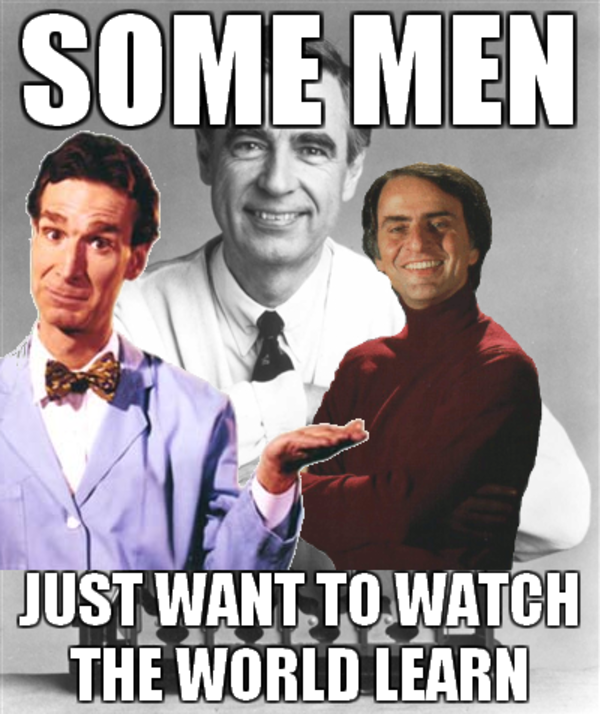
\includegraphics[width=0.4\textwidth]{images/watchandlearn.png}
\end{center}

\end{frame}

\begin{frame}
\frametitle{Remember the Initial Quiz}


Think back: what operations are fast and what operations are not?

Takeaway: our intuition  is often wrong. 

Not just at a macro level, but at a micro level. 

You may be able to narrow down that this computation of $x$ is slow, \\
but if you examine it carefully\ldots what parts of it are slow?


\end{frame}



\begin{frame}
\frametitle{Premature Optimization}

\vspace*{.5cm}

\begin{quote}
\textit{Programmers waste enormous amounts of time thinking about, or worrying about, the speed of noncritical parts of their programs, and these attempts at efficiency actually have a strong negative impact when debugging and maintenance are considered. We should forget about small efficiencies, say about 97\% of the time: premature optimization is the root of all evil. Yet we should not pass up our opportunities in that critical 3\%.}
\end{quote}
	\hfill -- Donald Knuth


\end{frame}



\begin{frame}
\frametitle{That Saying You Were Expecting}


Feeling lucky? \\
Maybe you optimized a slow part. 

\begin{center}
	\includegraphics[width=0.4\textwidth]{images/feellucky.jpg}
\end{center}

To make your programs or systems fast, \\
you need to find out what is currently slow and improve it (duh!). 

Up until now, it's mostly been about \\
\qquad ``let's speed this up''.\\
We haven't taken much time to decide what we should speed up.

\end{frame}


\begin{frame}
\frametitle{Why Observation?}

\begin{center}
	
\includegraphics[width=0.5\textwidth]{images/observe.jpg}
\end{center}

Observation is a bit more than just measuring things.

\end{frame}


\begin{frame}
\frametitle{Kinds of Observation}

\begin{enumerate}
	\item Counters
	\item Profiles
	\item Traces
\end{enumerate}

We'll return to profiling later on.

\end{frame}


\begin{frame}
\frametitle{Tracing: Logging}

Logging is an effective way of finding out what's happening.

We have surely all used \texttt{printf} to debug!

Logs need: timestamp, message, \& attributes.

\end{frame}


\begin{frame}
\frametitle{Logging} 

If we get only one tool -- logging!

How often to log, and what content?

This may be our only shot to get that info...\\
\quad But don't drown out relevant things!


\end{frame}


\begin{frame}
\frametitle{Ideas}

Log input and output?

Want to be able to link things...


\end{frame}


\begin{frame}[fragile]
\frametitle{Example}

{\scriptsize
\begin{verbatim}
Received request: update plan of company 12345 to ULTIMATE
Retrieving company 12345
Verifying eligibility for upgrade of company 12345 from BASIC to ULTIMATE
Company 12345 is not eligible for upgrade due to: unpaid invoices > 0
Returning response: update of company 12345 to ULTIMATE is DECLINED
\end{verbatim}
}

\end{frame}


\begin{frame}
\frametitle{Timestamp Precision}

Timestamp precision depends on the timescale of execution.

Time zones matter. Recommendation: UTC!

Or Stardates?

\begin{center}
	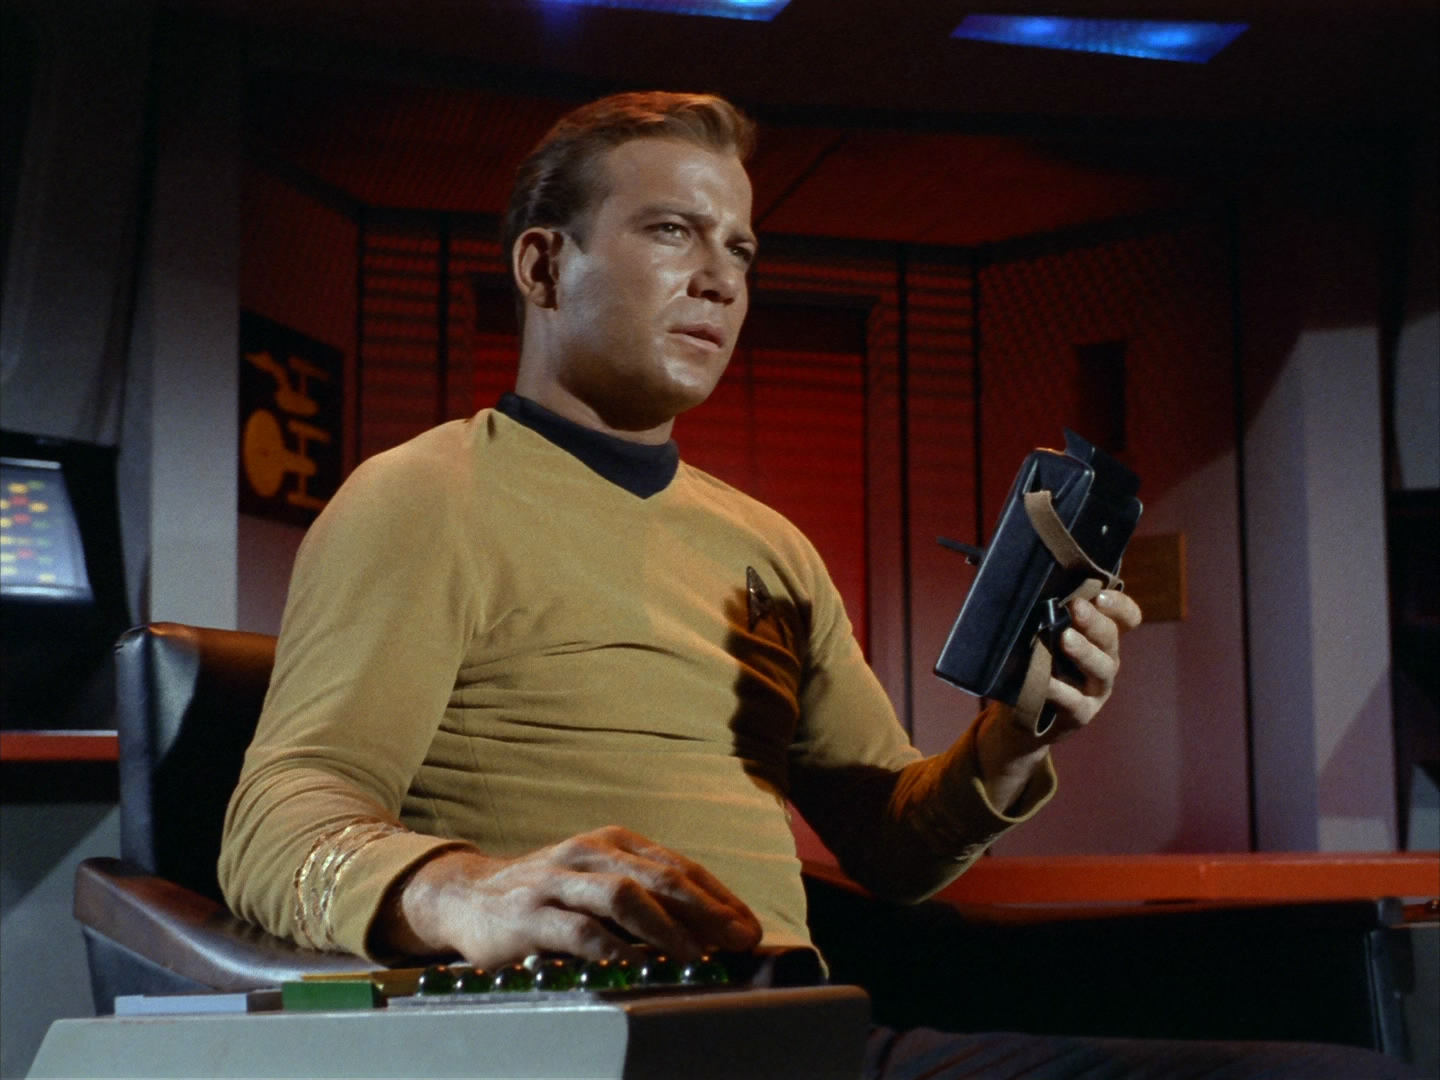
\includegraphics[width=0.4\textwidth]{images/captainslog.jpg}
\end{center}

\end{frame}


\begin{frame}
\frametitle{Too Much Noise}

Logging every request might be too noisy.

Searching and sorting help!

Too much detail is also bad...

\end{frame}


\begin{frame}
\frametitle{Personally Identifiable Information = No}

\begin{center}
	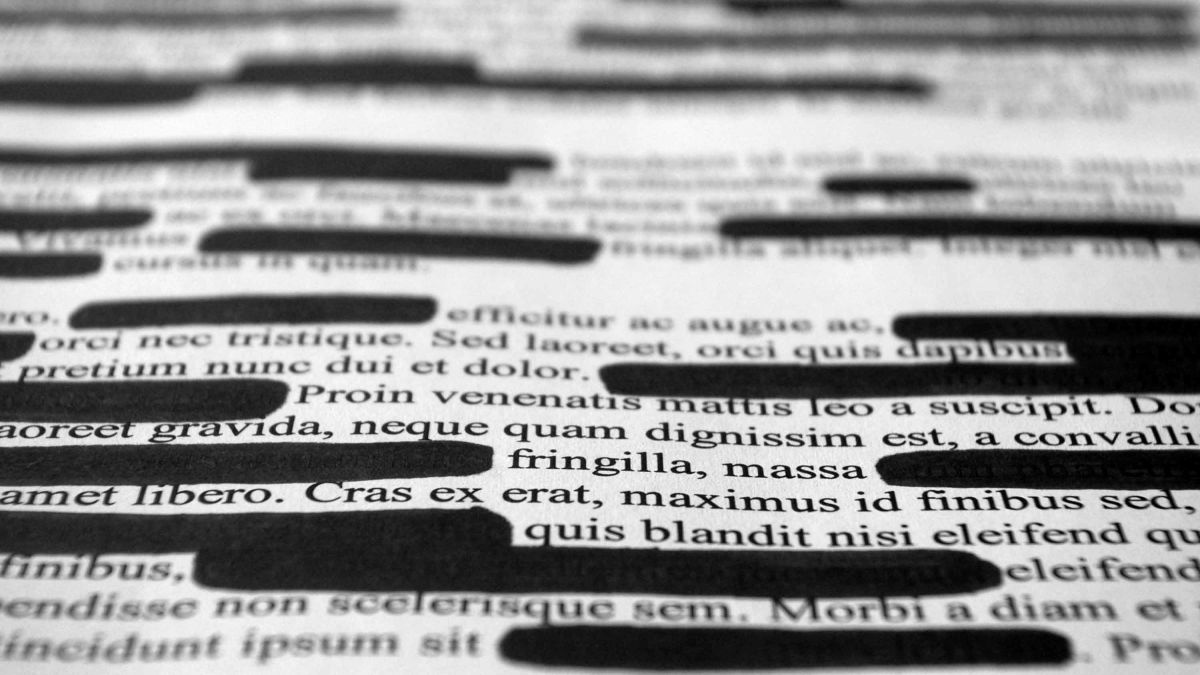
\includegraphics[width=\textwidth]{images/redacted.jpg}
\end{center}

\end{frame}


\begin{frame}
\frametitle{Over-logging}

Is it too hard to get access to info other ways?

Aim for a balance.


\end{frame}


\begin{frame}
\frametitle{Overhead of Tracing}

CPU trace tool: $20\times$ slowdown.

Timestamp at function call: $1.2-1.5\times$ slowdown.

Timestamp of system call entry/exit: $< 1\%$

\end{frame}


\begin{frame}
\frametitle{Other Overhead Tracing}

Valgrind: Up to $100\times$ slowdown.

Disk trace: pretty minimal!

Can identify deadlocks and waiting for locks.

\end{frame}


\begin{frame}
\frametitle{Space, the Final Frontier}

\begin{center}
	
\includegraphics[width=0.3\textwidth]{images/finalfrontier.jpg}
\end{center}
\hfill Image Credit: Revma Mahita

The trace itself takes up space.

20 GB/s bandwidth and 64-byte cache lines recording up to 8 bytes of data per trace entry could result in producing data at a rate of 2.4 GB per second.

\end{frame}


\begin{frame}
\frametitle{Counters}

Counters, as the name suggests, keep a count of events: interrupts, cache misses, data bytes written, calls to function \texttt{do\_magic()}.


Counters are aggregation, because we're summing the number of occurrences.

\end{frame}


\begin{frame}
\frametitle{Other Aggregation}

Average response time is aggregation: total time and number of requests.

Asking the computer to calculate the summary is sensible.

Ideas: number of requests, requests broken down by type, average time to respond to a request, percentage of error responses...  


\end{frame}


\begin{frame}
\frametitle{Context is Key}

\begin{center}
	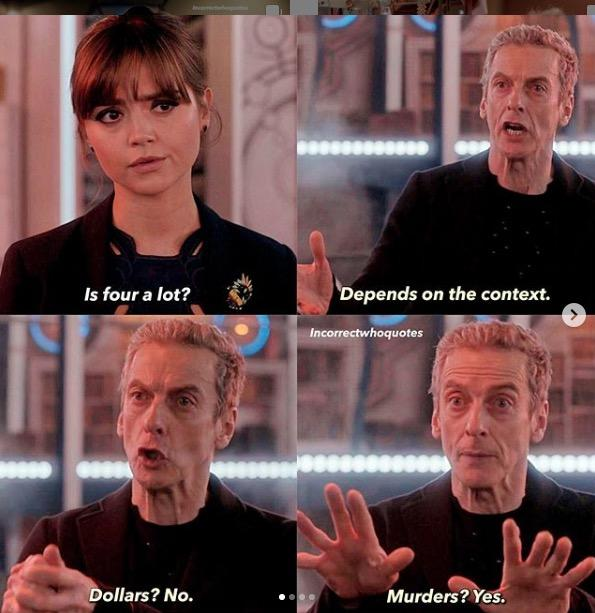
\includegraphics[width=0.6\textwidth]{images/context.jpg}
\end{center}


\end{frame}


\begin{frame}
\frametitle{Context to Aggregation}

After my PR, login time $0.75s$ -- Good or bad?

Depends on the baseline. Maybe it was $0.5s$?


Okay, increased -- is that bad?

\end{frame}


\begin{frame}
\frametitle{Another Example}

Request takes on average $1.27s$ -- Good or Bad?

What if the time limit is 1 second? 10 seconds?

How hard is the deadline?

\end{frame}


\begin{frame}
\frametitle{Averages Misleading}

All of these are 7 requests per second on average:

\begin{center}
	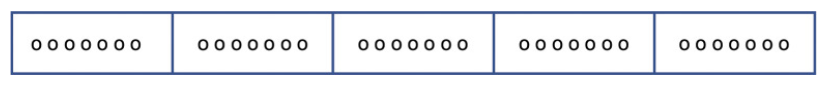
\includegraphics[width=\textwidth]{images/burst1}\\
	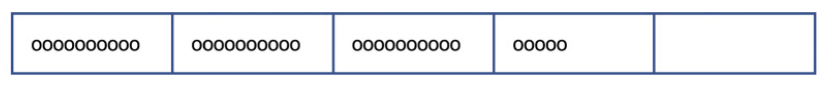
\includegraphics[width=\textwidth]{images/burst2}\\
	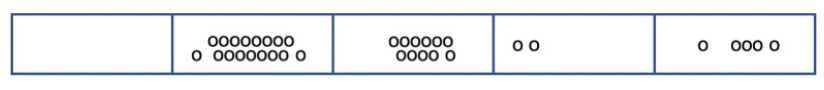
\includegraphics[width=\textwidth]{images/burst3}\\
\end{center}


\end{frame}

\begin{frame}
\frametitle{Time Period}

When we aggregate, we have to choose the period of time.

Whole execution of the task?

Indefinitely-running services?

We might miss important things!

\end{frame}


\begin{frame}
\frametitle{Look at the Pretty Pictures}

Graphs and visualizations help us see trends in data.

\begin{center}
	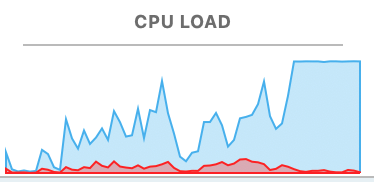
\includegraphics[width=0.7\textwidth]{images/cpu-load.png}
\end{center}

Managers and non-techies love them!

If we put together enough pretty pictures, we get a dashboard.

\end{frame}


\begin{frame}
\frametitle{Dashboards}

Dashboards are ideally more than just pretty pictures of LINE GOES UP.

\begin{center}
	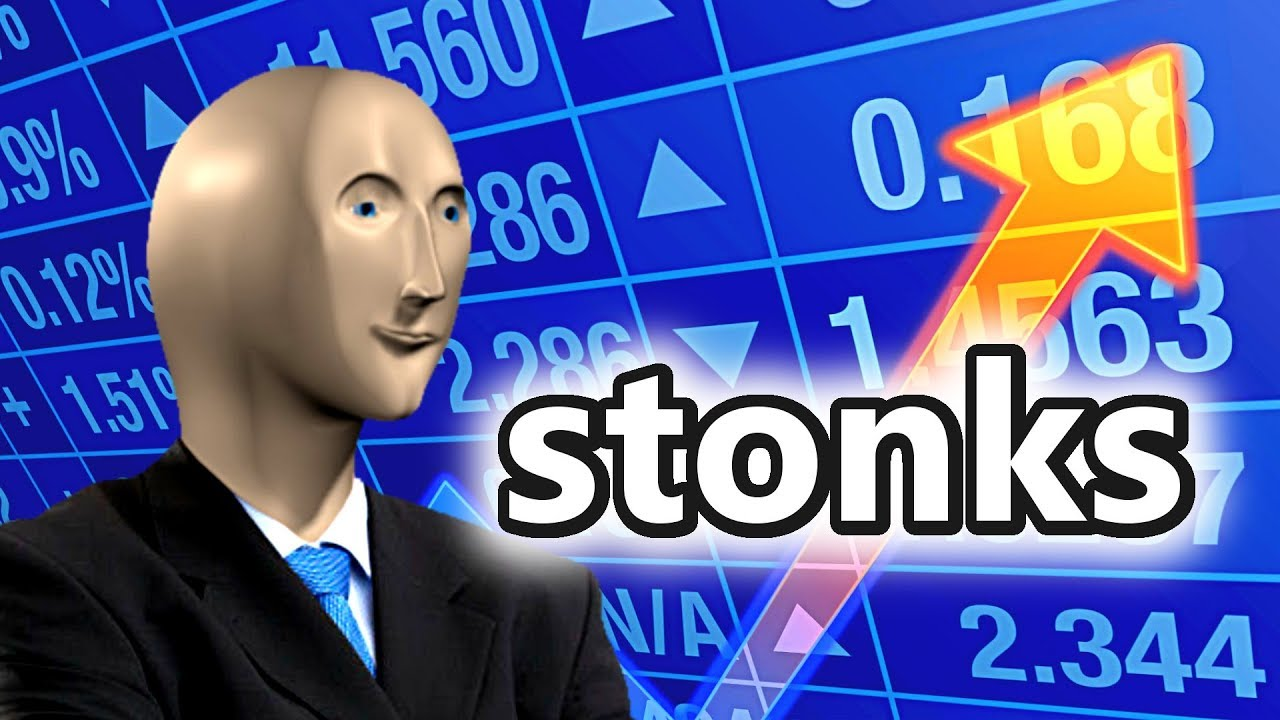
\includegraphics[width=\textwidth]{images/stonks.jpg}
\end{center}

Should present an easily-digestible summary.

\end{frame}


\begin{frame}
\frametitle{Drill Down}

This is just a high level idea of identifying what's happening.

As we proceed we need to get to lower level tools.

Next: narrowing down where the bottleneck is.

\end{frame}






\end{document}

